\documentclass{beamer}
\usetheme{Malmoe}


\usepackage{graphicx}
\usepackage{fontspec}
\setsansfont{楷体}


\begin{document}

\title[\sc Ray-Traing based Renderer]{\sc 基于光线追踪(Ray-Tracing) \\ 原理的物理渲染器实现}
\author{ \normalsize 余畅(95) \quad \tiny (2019091621002) \\
 \normalsize 张清安(92) \qquad \tiny (2019091621014) \\
 \normalsize 伍桐雨(92) \quad \tiny (2019091619028) \\
 \normalsize 肖荣博(92) \quad \tiny (2019091621017)}
\date{\today}
\institute[UESTC]{Software Engeering, UESTC}
\frame{\titlepage}

\section{Requirement}
\begin{frame} {需求分析}
		\begin{itemize} [<+->]
\item 渲染(Render)指将三维场景中的模型,按照设定好的 \\ 环境、灯光、材质及渲染参数,二维投影成数字图像的过程。
\item 光线追踪技术(Ray-Tracing)是由几何光学衍生而来。 它通过追踪光线与物体表面发生的 \\ 交互作用,得到光线经过路径的模型。
\item 本项目旨在通过已学的线代和微积分知识,\\实现一个简易的光追渲染器
\end{itemize}
\end{frame}

\section{Samples}
\begin{frame} {Samples 1}
\normalsize The Cornell Box \tiny (data from graphics.cornell.edu) \\
\normalsize The Stanford Bunny \tiny (Source: Stanford University Computer Graphics Laboratory) \\
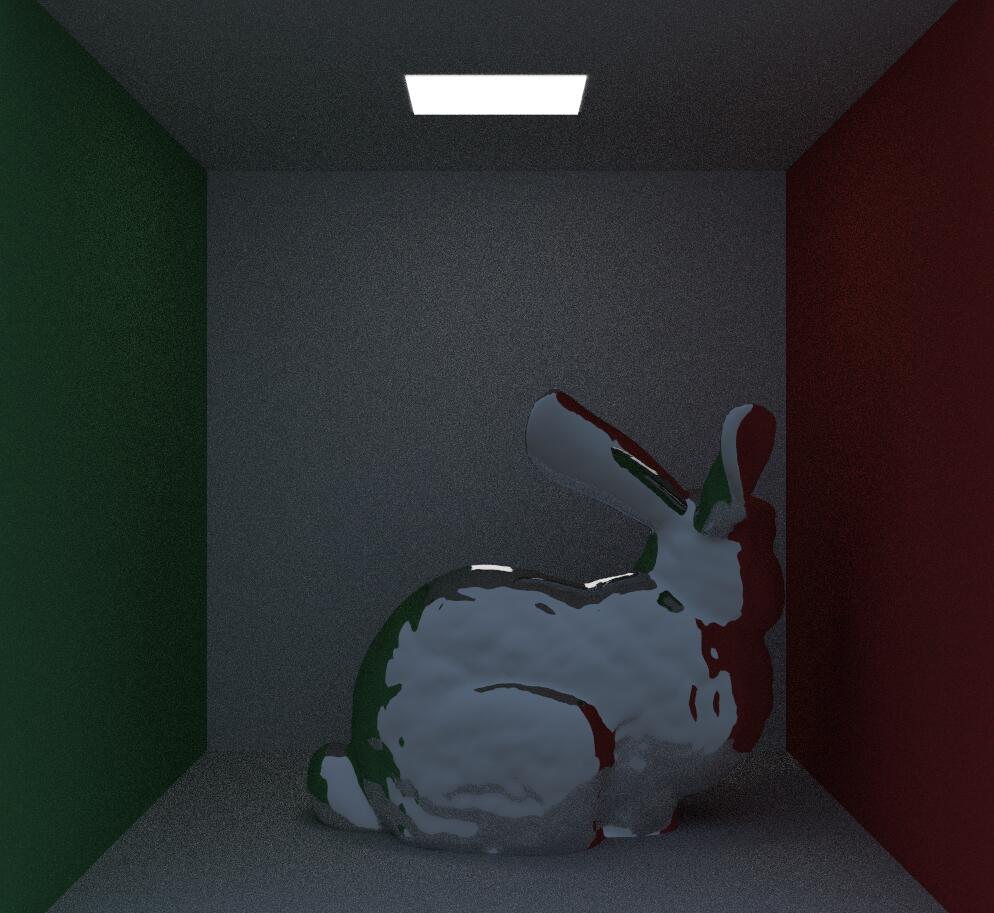
\includegraphics[scale=0.25]{bunny.jpg}
\tiny (600x600 500 samples per pixel) \\
\end{frame}

\begin{frame} {Samples 2}
\normalsize spheres \tiny (data from random generator) \\
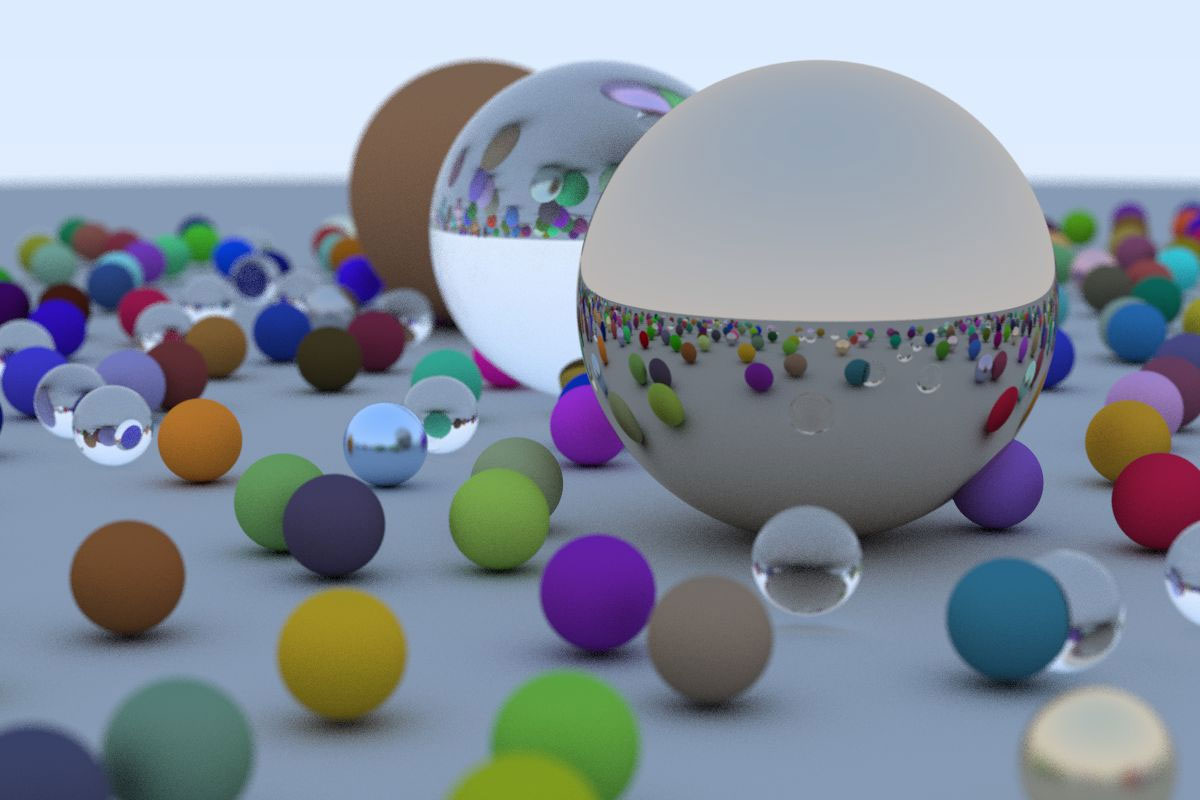
\includegraphics[scale=0.2]{balls.jpg} \\
\tiny (1200x900 500 samples per pixel) \\
\end{frame}

\begin{frame} {Samples 3}
\normalsize Happy Buddha \tiny (Source: Stanford University Computer Graphics Laboratory) \\
\normalsize Lambertian material \\
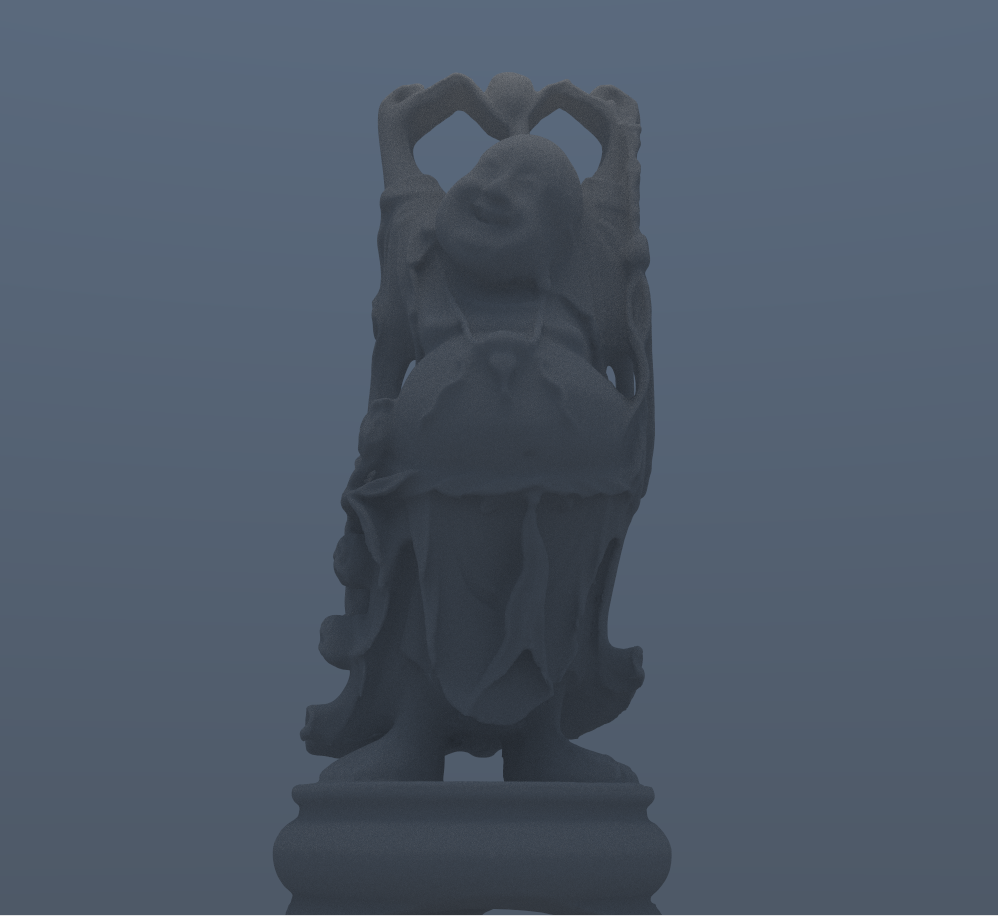
\includegraphics[scale=0.18]{buda.png}
\tiny (900x900 1000 samples per pixel) \\
\end{frame}

\label{section2}
\begin{frame} {Samples 4}
\normalsize The Stanford Bunny \tiny (Source: Stanford University Computer Graphics Laboratory) \\
\normalsize Dielectric material \\
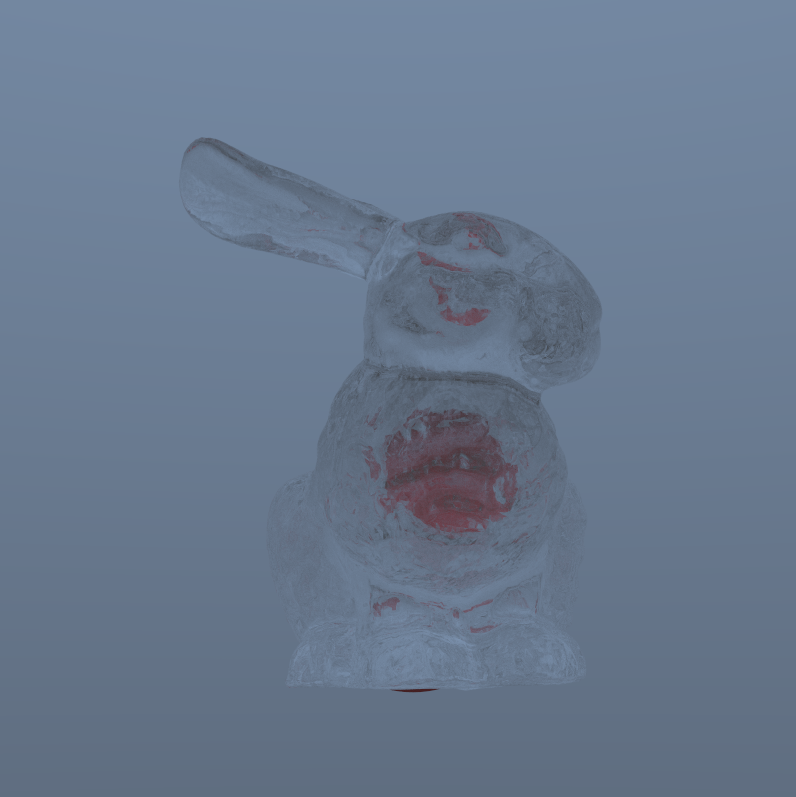
\includegraphics[scale=0.18]{glassbunny.png}
\tiny (900x900 300 samples per pixel) \\
\end{frame}

\section{Linear algebra library}
\begin{frame} {模块 1: 底层线性代数数学库 (张清安,肖荣博) }
\begin{block}{主要功能}
    提供常用线性代数中 \\ 数学量(点,向量,法线,矩阵) 的结构体和 \\ 运算方法 (线性运算,数乘,内外积,\\ 矩阵的转置,求逆,乘法等)的函数
  \end{block}
\begin{itemize}
			\item \begin{semiverbatim}
    ./math/vector3.h
  \end{semiverbatim}
			\item \begin{semiverbatim}
    ./math/matrix3x3.h
  \end{semiverbatim}
			\item \begin{semiverbatim}
    ./math/transform.h
  \end{semiverbatim}
\item \begin{semiverbatim}
    ./math/quaternion.h
  \end{semiverbatim}
\end{itemize}
\end{frame}

\begin{frame} {/math/vector3.h}
\begin{itemize} [<+->]
\item 实现了Normal3, Point3, Vector3类
\item 为了方便调用,运算符重载了线性运算
\begin{semiverbatim} \small BaseVector3 operator + (const BaseVector3 \&v) const; \end{semiverbatim}
\begin{semiverbatim} \small friend BaseVector3 operator * (const float \&s, const BaseVector3 \&v); \end{semiverbatim}
\begin{semiverbatim} \small ... \end{semiverbatim}
\item 实现了点积,叉积,求长度,求距离,标准化等方法
\begin{semiverbatim} \small float dot(const BaseVector3 \&v) const; \end{semiverbatim}
\begin{semiverbatim} \small float length() const; \end{semiverbatim}
\begin{semiverbatim} \small float distance(const BaseVector3 \&p) const; \end{semiverbatim}
\begin{semiverbatim} \small BaseVector3\& normalize(); \end{semiverbatim}
\begin{semiverbatim} \small ... \end{semiverbatim}
\end{itemize}
\end{frame}

\begin{frame} {/math/vector3.h}
\begin{itemize} [<+->]
\item SIMD(Single Instruction Multiple Data)
\item 单指令多数据流,能够复制多个操作数,\\并把它们打包在大型寄存器的一组指令集。
\item 向量每个分量在线性运算时候都是独立的,\\ 可以依靠SIMD并行运算
\item 本项目通过intrin.h,实现了X86平台下的SIMD优化
\item \begin{semiverbatim} ... \newline \_\_m128 vs = \_mm\_load\_ss(\&s); \newline vs = \_mm\_pshufd\_ps(vs, 0x80); \newline m\_val128 = \_mm\_mul\_ps(m\_val128, vs); \newline ... \end{semiverbatim}
\end{itemize}
\end{frame}

\begin{frame} {/math/matrix3x3.h}
\begin{itemize} [<+->]
\item 实现了Matrix3x3类
\item 用三个vector3表示一个3x3的矩阵
\item 实现了矩阵的常用运算
\begin{semiverbatim} \small Matrix3x3 transpose() const; \end{semiverbatim}
\begin{semiverbatim} \small Matrix3x3 absolute() const; \end{semiverbatim}
\begin{semiverbatim} \small Matrix3x3 adjoin() const; \end{semiverbatim}
\begin{semiverbatim} \small Matrix3x3 inverse() const; \end{semiverbatim}
\begin{semiverbatim} \small ... \end{semiverbatim}
\end{itemize}
\end{frame}

\begin{frame} {/math/transform.h}
\begin{itemize} [<+->]
\item 实现了Transform类
\item 封装了一个Matrix3x3和Vector3及其逆过程,\\ 表达了空间中的一个变换
\begin{semiverbatim} \small [Transform class members:] \end{semiverbatim}
\begin{semiverbatim} \small Matrix3x3 m\_mat, m\_inv; \end{semiverbatim}
\begin{semiverbatim} \small Vector3 m\_trans; \end{semiverbatim}
\end{itemize}
\end{frame}

\begin{frame} {位移 (Translate)}
		\begin{itemize}
\item $m\_trans = (x, y, z) $
\item 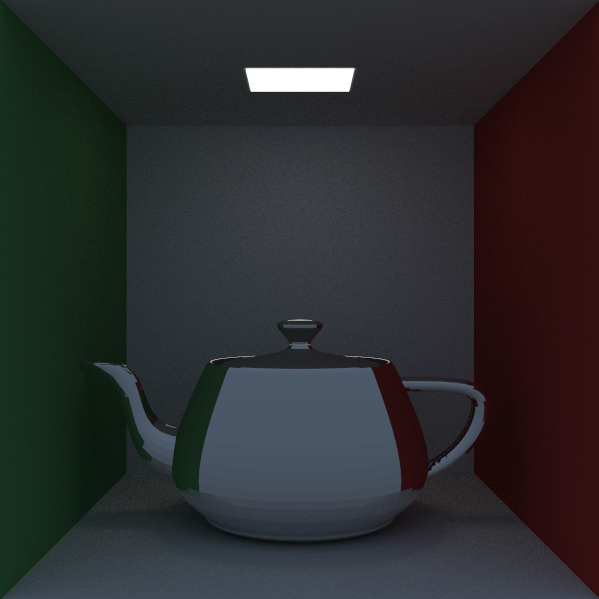
\includegraphics[scale=0.2]{cornellbox_teapot_common} To 
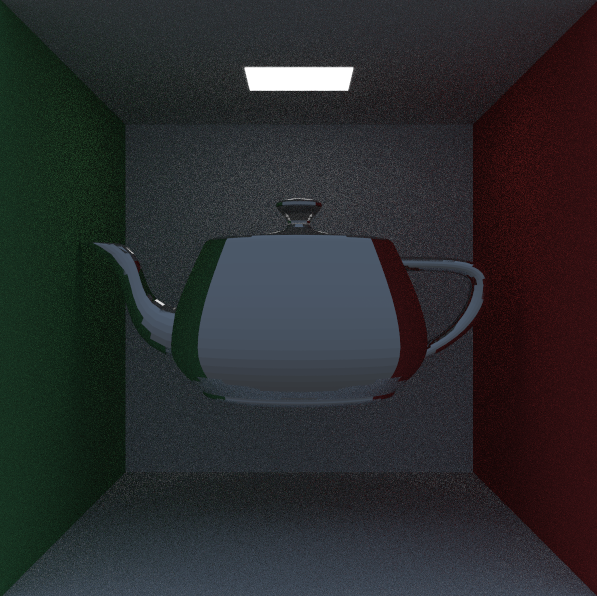
\includegraphics[scale=0.2]{cornellbox_teapot_translate}
\end{itemize}
\end{frame}

\begin{frame} {缩放 (Scale)}
\begin{itemize}
\item $m\_mat = \begin{bmatrix} x&0&0\\ 0&y&0\\ 0&0&z \end{bmatrix} ,m\_mat^{-1} = \begin{bmatrix} \frac{1}{x}&0&0\\ 0&\frac{1}{y}&0\\ 0&0&\frac{1}{z} \end{bmatrix}$
\item 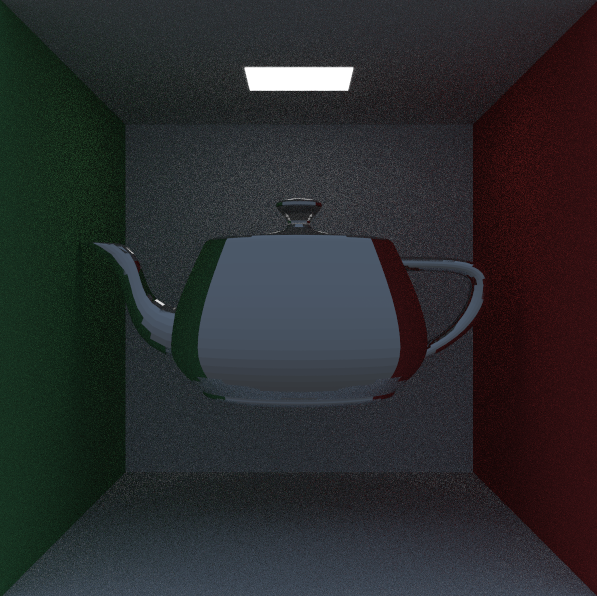
\includegraphics[scale=0.2]{cornellbox_teapot_translate} To 
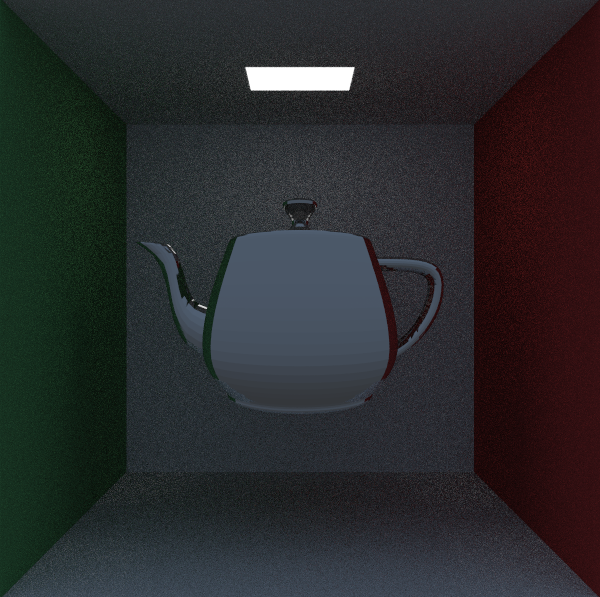
\includegraphics[scale=0.2]{cornellbox_teapot_scale}
\end{itemize}
\end{frame}

\begin{frame} {旋转 (Rotation)}
\begin{itemize}
\item 设旋转轴为$A$,旋转角为$\theta$, $c = cos\theta, s = sin\theta$
\item \tiny $m\_mat = \begin{bmatrix} c+(1-c)A_x^2&(1-c)A_xA_y-sA_z&(1-c)A_xA_z+sA_y\\ (1-c)A_xA_y&c+(1-c)A_y^2&(1-c)A_xA_y-sA_z\\ (1-c)AxAz-sA_y&(1-c)A_yA_z+sA_x&c+(1-c)A_z^2 \end{bmatrix} ,m\_mat^{-1} = m\_mat^T$
\item 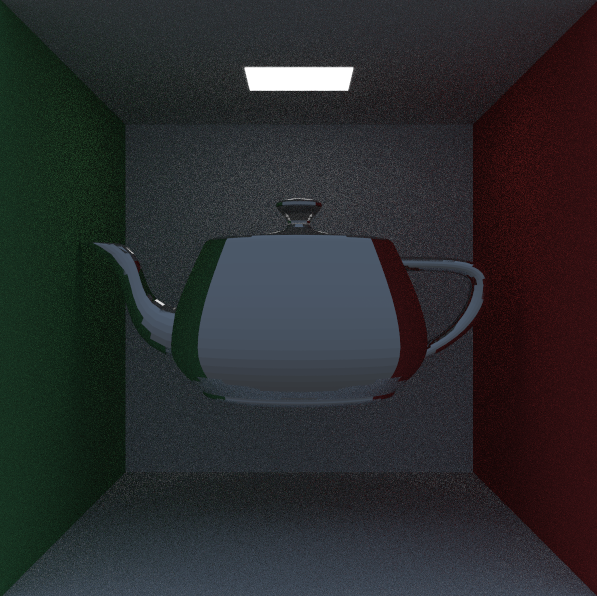
\includegraphics[scale=0.2]{cornellbox_teapot_translate} \normalsize To 
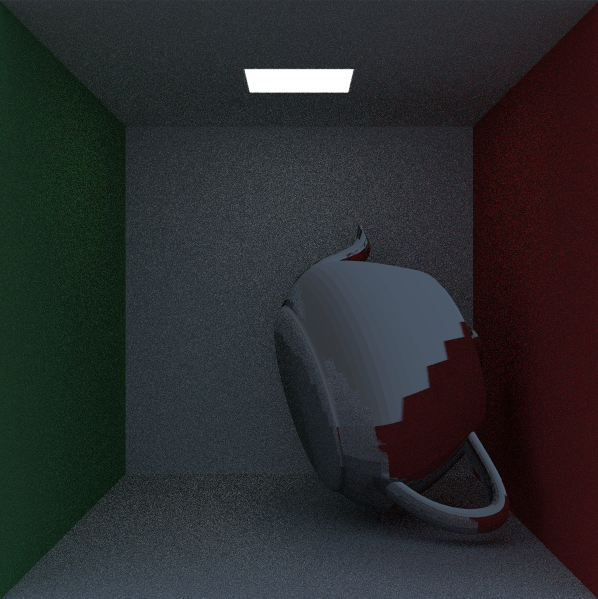
\includegraphics[scale=0.2]{cornellbox_teapot_rotate}
\end{itemize}
\end{frame}

\section{Ray-Tracing implement}
\begin{frame} {模块 2: 光追渲染器组件实现 (余畅) }
\begin{block}{主要功能}
    定义场景中的物体,材质,纹理相机等参数,\\ 并实现光线传播(漫反射,镜面反射,折射,相交)的相应计算
  \end{block}
\begin{itemize}
			\item \begin{semiverbatim}
    ./core/camera.h
  \end{semiverbatim}
			\item \begin{semiverbatim}
    ./core/integrator.h
  \end{semiverbatim}
			\item \begin{semiverbatim}
    ./core/material.h
  \end{semiverbatim}
\item \begin{semiverbatim}
    ./core/primitive.h,cpp
  \end{semiverbatim}
\item \begin{semiverbatim}
    ./core/texture.h
  \end{semiverbatim}
\item \begin{semiverbatim}
    ./shapes/rectangle.h,cpp
  \end{semiverbatim}
\item \begin{semiverbatim}
    ./shapes/sphere.h,cpp
  \end{semiverbatim}
\item \begin{semiverbatim}
     ./shapes/triangle.h,cpp
  \end{semiverbatim}
\item \begin{semiverbatim}
    ./accelerators/BVH.h,cpp
  \end{semiverbatim}
\end{itemize}
\end{frame}

\begin{frame} {/core/camera.h}
\begin{itemize} [<+->]
\item 实现了Camera, ProjectiveCamera类
\item Camera必须实现的方法
\begin{semiverbatim} virtual Ray getRay(const float \&s, const float \&t) const; \end{semiverbatim}
\item 投影相机(ProjectiveCamera类)
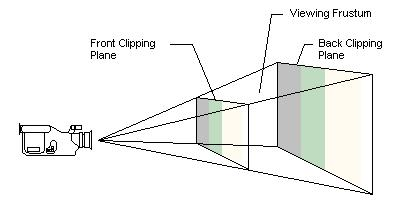
\includegraphics[scale=1]{projectivecamera.jpg}
\end{itemize}
\end{frame}

\begin{frame} {/core/camera.h}
\begin{itemize}
\item 
\begin{semiverbatim} const Point3 lookform, \newline const Point3 lookat, \newline const Vector3 vup \end{semiverbatim}
确定了摄像机的位置和角度
\item 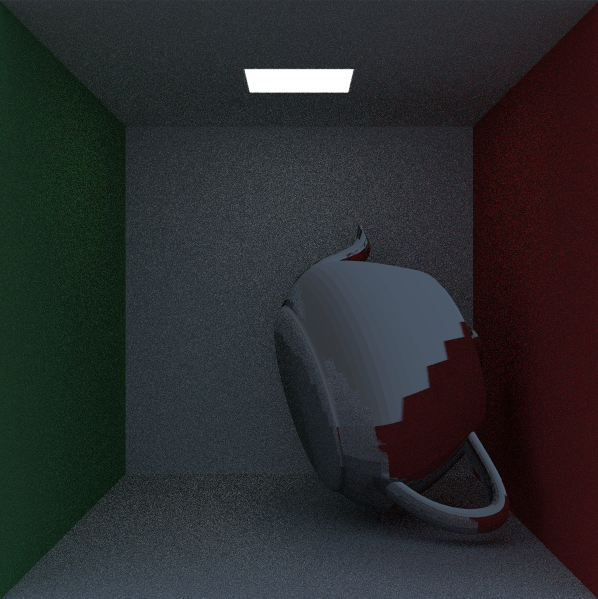
\includegraphics[scale=0.2]{cornellbox_teapot_rotate} \normalsize To 
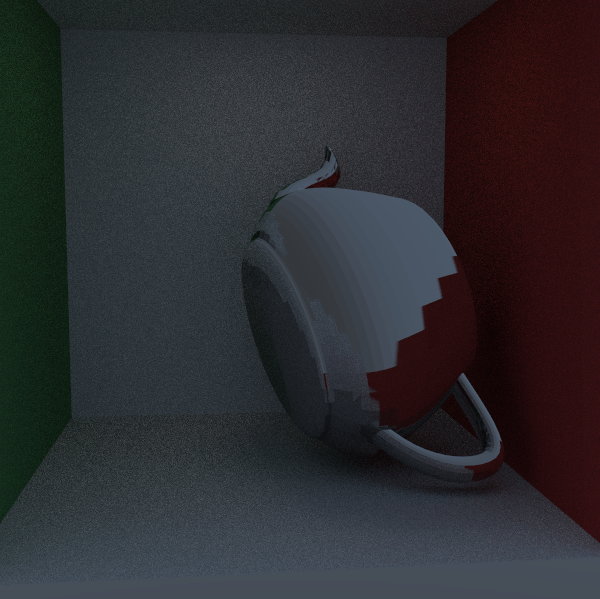
\includegraphics[scale=0.2]{cornellbox_teapot_camera_move}
\end{itemize}
\end{frame}

\begin{frame} {/core/camera.h}
\begin{itemize}
\item 
\begin{semiverbatim} float vfov \end{semiverbatim}
确定视角的大小
\item 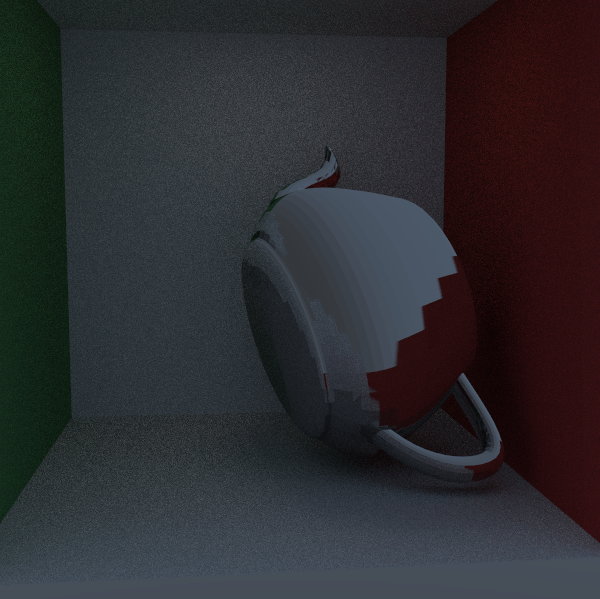
\includegraphics[scale=0.2]{cornellbox_teapot_camera_move} \normalsize To 
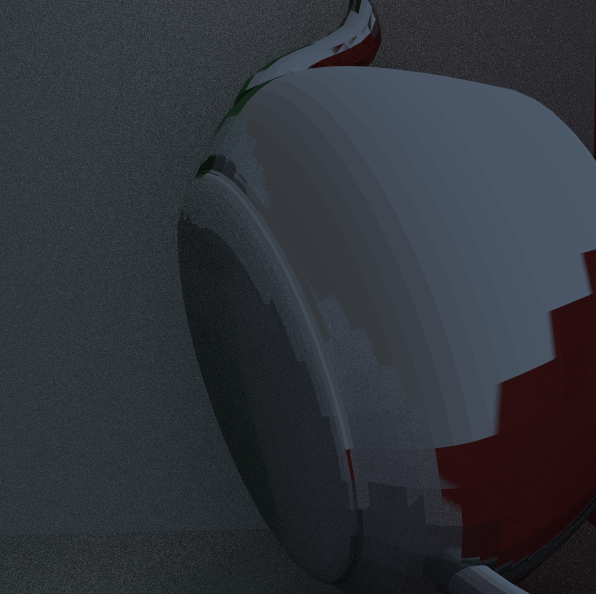
\includegraphics[scale=0.2]{cornellbox_teapot_camera_fov}
\end{itemize}
\end{frame}

\begin{frame} {/core/camera.h}
\begin{itemize}
\item 
\begin{semiverbatim} float aperture \end{semiverbatim}
确定光圈(小孔成像中小孔)的半径
\item 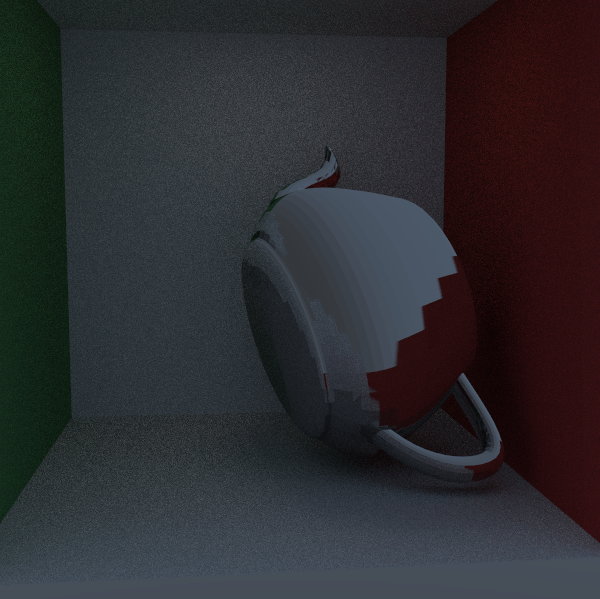
\includegraphics[scale=0.2]{cornellbox_teapot_camera_move} \normalsize To 
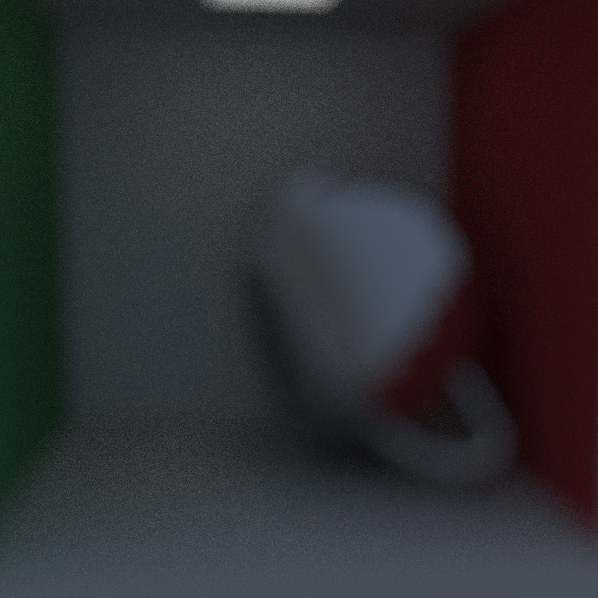
\includegraphics[scale=0.2]{cornellbox_teapot_blur}
\end{itemize}
\end{frame}

\begin{frame} {/core/texture.h}
\begin{itemize} [<+->]
\item 实现了Texture, ConstantTexture, CrossTexture, NoiseTexture类
\item Texture必须实现的方法
\begin{semiverbatim} virtual Spectrum value(float u, float v, const Point3 \&p) const; \end{semiverbatim}
对通过光线与平面交点及$(u, v)$坐标对纹理采样颜色
\end{itemize}
\end{frame}

\begin{frame} {/core/texture.h}
\begin{itemize}
\item ConstantTexture,返回一个常量颜色的纹理
\item 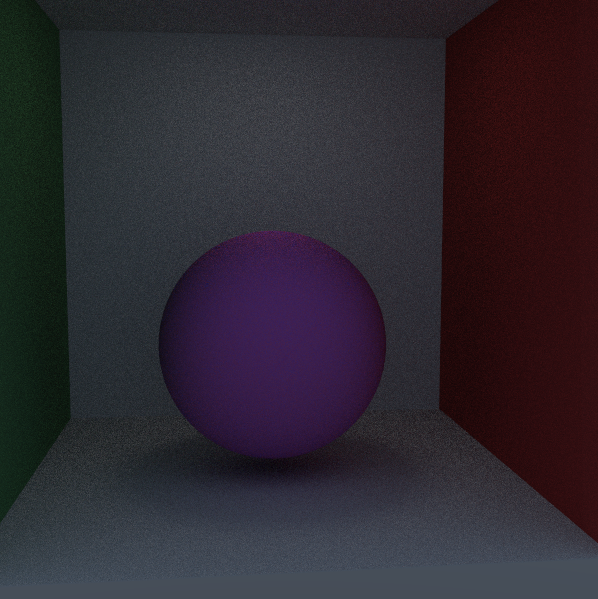
\includegraphics[scale=0.2]{constant}
\end{itemize}
\end{frame}

\begin{frame} {/core/texture.h}
\begin{itemize}
\item CrossTexture,返回一个交错的棋盘纹理
\item 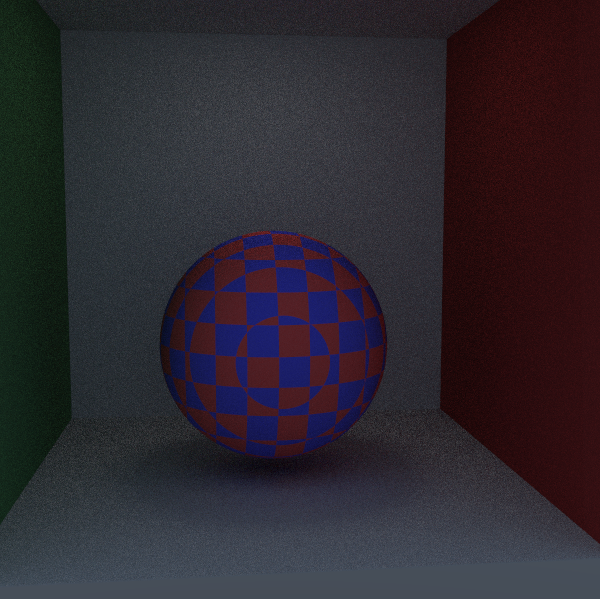
\includegraphics[scale=0.2]{cross}
\end{itemize}
\end{frame}

\begin{frame} {/core/texture.h}
\begin{itemize}
\item NoiseTexture,返回一个柏林噪音(Perlin Noise)实现的随机纹理
\begin{figure}[htbp]
\centering
\begin{minipage}[t]{0.4\textwidth}
\centering
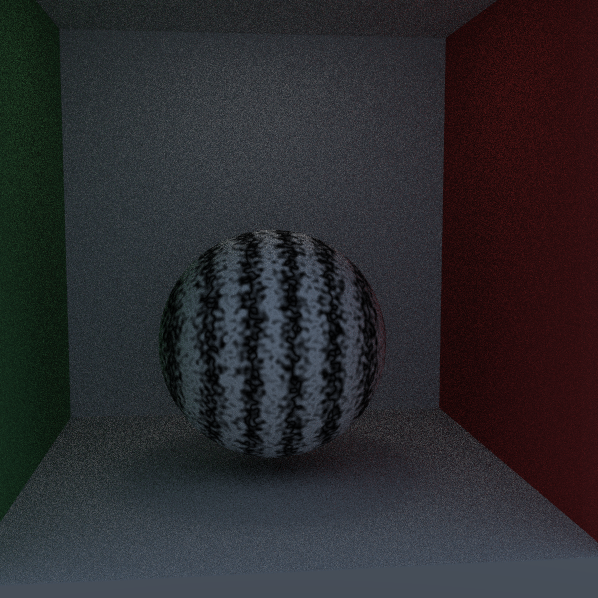
\includegraphics[width=4cm]{noise2}
\caption{scale = 0.5}
\end{minipage}
\begin{minipage}[t]{0.4\textwidth}
\centering
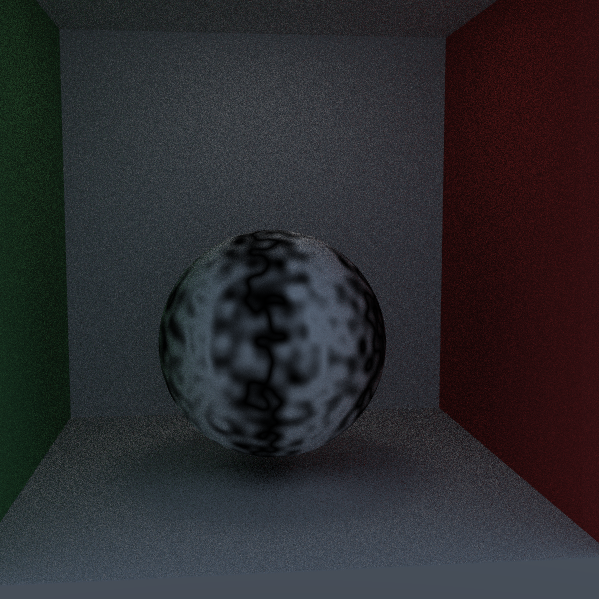
\includegraphics[width=4cm]{noise3}
\caption{scale = 0.05}
\end{minipage}
\end{figure}
\end{itemize}
\end{frame}

\begin{frame} {/core/material.h}
\begin{itemize} [<+->]
\item 实现了Material, MentalMaterial, LambertianMaterial, DielectricMaterial类
\item Material必须实现的方法
\begin{semiverbatim} \small virtual bool scatter \newline (const Ray \&r\_in, const SurfaceInteraction \&si, Spectrum \&attenuation, Ray \&scattered) const; \end{semiverbatim}
根据入射光线和表面的信息,返回出射光线和衰减率
\item 
\begin{semiverbatim} \small virtual Spectrum emitted \newline (float u, float v, const Vector3 \&p) const; \end{semiverbatim}
返回物体的自发光
\end{itemize}
\end{frame}

\begin{frame} {/core/material.h}
\begin{itemize}
\item LambertianMaterial,漫反射材质
\item 光线射入物体后向各方向随机漫反射
\begin{semiverbatim} \small Vector3 target = si.p + si.n + rng.randomInUnitSphere(); \end{semiverbatim}
\begin{semiverbatim} \small scattered = Ray(si.p, target - si.p, r\_in.m\_time); \end{semiverbatim}
\item 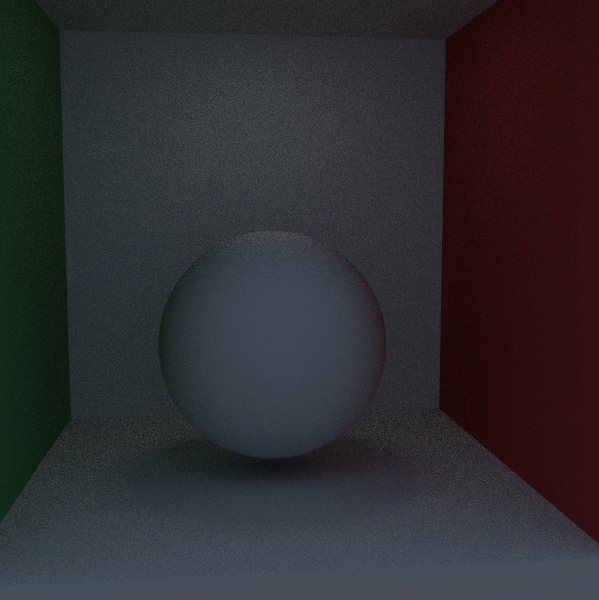
\includegraphics[scale=0.2]{lamb}
\end{itemize}
\end{frame}

\begin{frame} {/core/material.h}
\begin{itemize}
\item MentalMaterial,金属材质
\item 入射角和反射角相同,即按法线反转
\item $out=in - (in,n) \cdot 2 \cdot n $
\item fuzz参数描述镜面的粗糙程度
\item 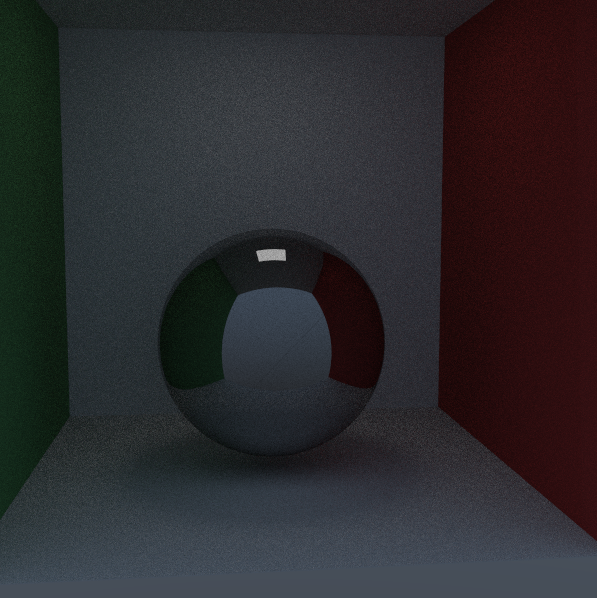
\includegraphics[scale=0.2]{mental}
\end{itemize}
\end{frame}

\begin{frame} {/core/material.h}
\begin{itemize}
\item DielectricMaterial,电介质材质
\item 同时存在镜面反射和折射效应,能量分配通过菲涅耳公式(Fresnel Formula)计算,实际项目中采用schlick公式近似
\item $\frac{sin \theta 1}{sin \theta 2} = r$
\item m\_refractive\_idx参数描述介质材料的折射率
\item 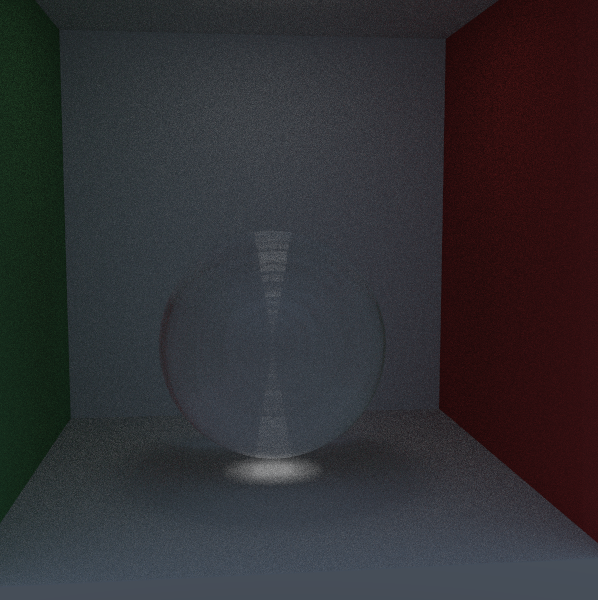
\includegraphics[scale=0.15]{glass}
\end{itemize}
\end{frame}

\begin{frame} {/core/shape.h}
\begin{itemize} [<+->]
\item 实现了Shape基类
\item Shape必须实现的方法
\item
\begin{semiverbatim} \small virtual BBox objectBound() const = 0; \end{semiverbatim}
返回形状在物体参考系中的包围盒
\item
\begin{semiverbatim} \small virtual BBox worldBound() const = 0; \end{semiverbatim}
返回形状在世界参考系中的包围盒
\item
\begin{semiverbatim} \small virtual bool canIntersect() const; \end{semiverbatim}
判断当前图元是否能相交
\item
\begin{semiverbatim} \small virtual void refine(std::vector<SharedPtr<Shape>>\&refined) const; \end{semiverbatim}
细分无法相交的图元
\item
\begin{semiverbatim} \small virtual bool intersect(const Ray \&ray, float *hit\_t, SurfaceInteraction *dg) const; \end{semiverbatim}
对相应光线执行相交计算
\end{itemize}
\end{frame}

\begin{frame} {/core/shape.h}
\begin{itemize} [<+->]
\item ./shapes/triangle.h
\item ./shapes/triangle.cpp
\item 为保证内存的连续性,三角形的顶点,索引等数据统一储存在 \\ TriangleMesh类中,具体计算由细分后的Triangle类实现
\item 相交方法实现以Fast, Minimum Storage Ray-Triangle Intersection为参考
\item 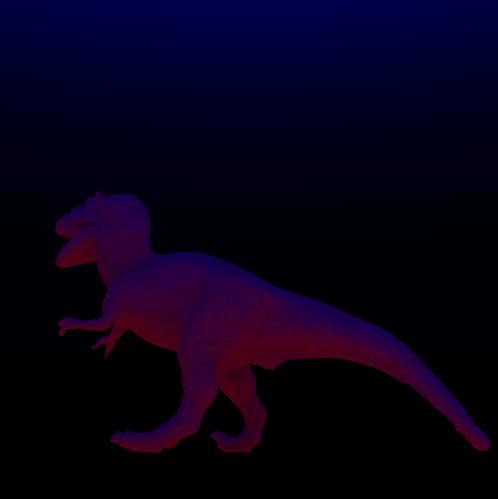
\includegraphics[scale=0.25]{tyra}
\end{itemize}
\end{frame}

\begin{frame} {/core/shape.h}
\begin{itemize} [<+->]
\item ./shapes/sphere.h
\item ./shapes/sphere.cpp
\item 计算相交即解一个关于射线参数t的一元二次方程
\item 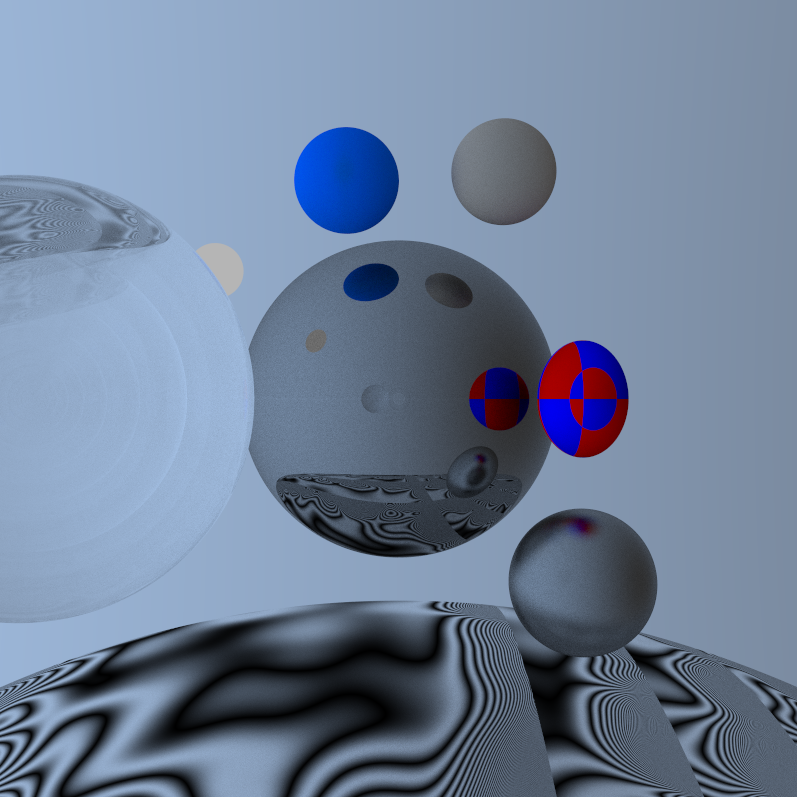
\includegraphics[scale=0.20]{spheres}
\end{itemize}
\end{frame}

\begin{frame} {/core/shape.h}
\begin{itemize} [<+->]
\item ./shapes/rectangle.h
\item ./shapes/rectangle.cpp
\item 将射线转化到物体坐标系后六个平面和坐标轴分别对齐,\\ 分别计算相交后取t的最小值的平面
\item 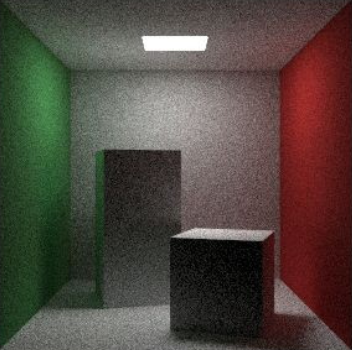
\includegraphics[scale=0.40]{rect}
\end{itemize}
\end{frame}

\begin{frame} {/accelerator/BVH.h}
\begin{itemize} [<+->]
\item 如果每一束光线都对场景中的每一个物体进行相交计算,\\ 计算开销将会无法接受
\item 本项目对每一个形状构建了包围盒,并使用了\\数据结构BVH(Bounding Volume Hierarchy)进行加速
\item 本质是一类二叉搜索树,每层对三条坐标轴中的一条进行排序
\item 复杂度可由$O(n^2)$降为$O(n log n)$
\end{itemize}
\end{frame}

\section{Parser}
\begin{frame} {模块 3: 场景描述文件解析器 (伍桐雨) }
\begin{block}{主要功能}
    实现了parser类,用以将描述场景的JSON文件和 \\ 描述模型的OBJ文件解析入Scene结构体的内存中
  \end{block}
\begin{itemize}
			\item \begin{semiverbatim}
    ./core/parser.h
  \end{semiverbatim}
			\item \begin{semiverbatim}
    ./core/parser.cpp
  \end{semiverbatim}
\end{itemize}
\end{frame}

\begin{frame} {/core/parser.h}
\begin{itemize} [<+->]
\item JSON(JavaScript Object Notation) 是一种轻量级的数据交换格式。易于人阅读和编写
\item JSON是一个标记符的序列。这套标记符包含六个构造字符、\\ 字符串、数字和三个字面名
\item 本项目使用的描述文件是JSON的子集,\\ 即parser类仅按照特定语法树和关键词进行解析
\end{itemize}
\end{frame}

\begin{frame} {/core/parser.h}
\begin{itemize}
\item
场景文件样例(part 1.) \\ 
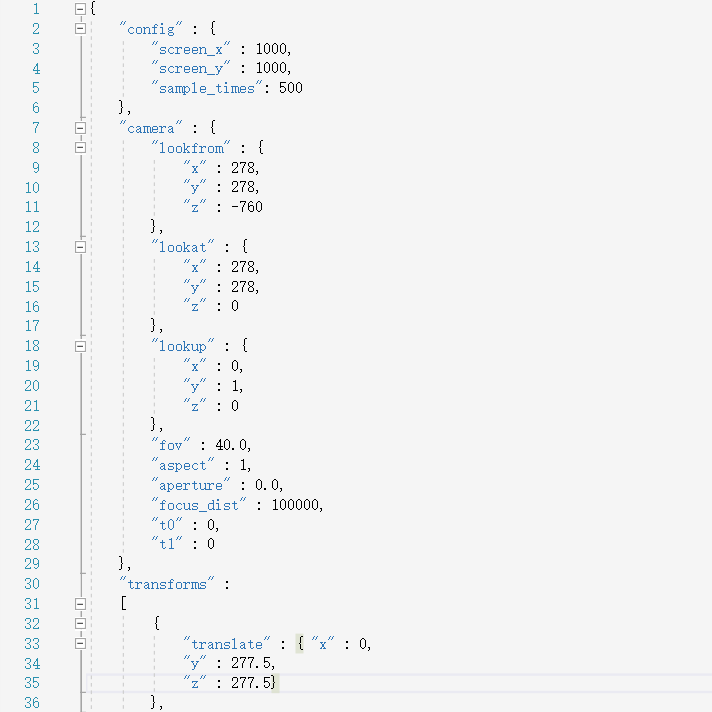
\includegraphics[scale=0.3]{code1}
\end{itemize}
\end{frame}

\begin{frame} {/core/parser.h}
\begin{itemize}
\item
场景文件样例(part 2.) \\ 
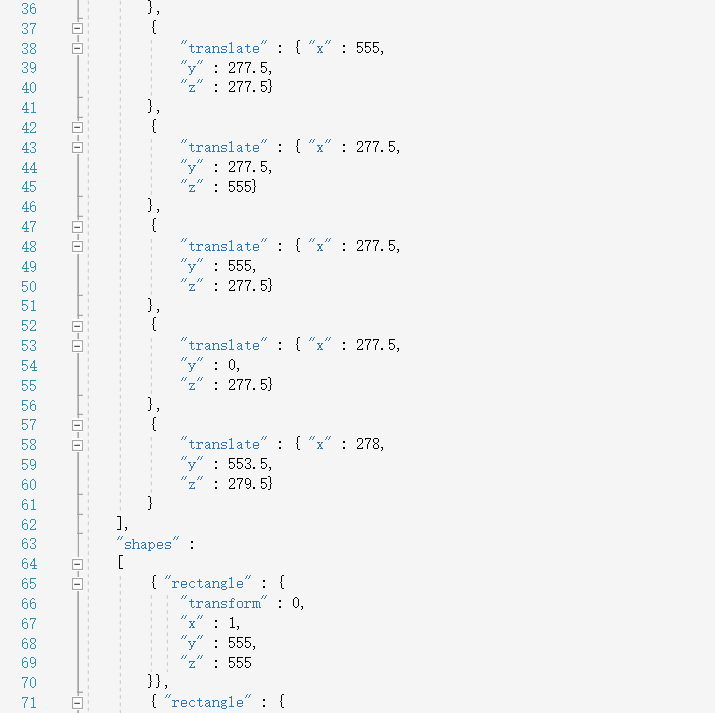
\includegraphics[scale=0.3]{code2}
\end{itemize}
\end{frame}

\begin{frame} {/core/parser.h}
\begin{itemize}
\item
场景文件样例(part 3.) \\ 
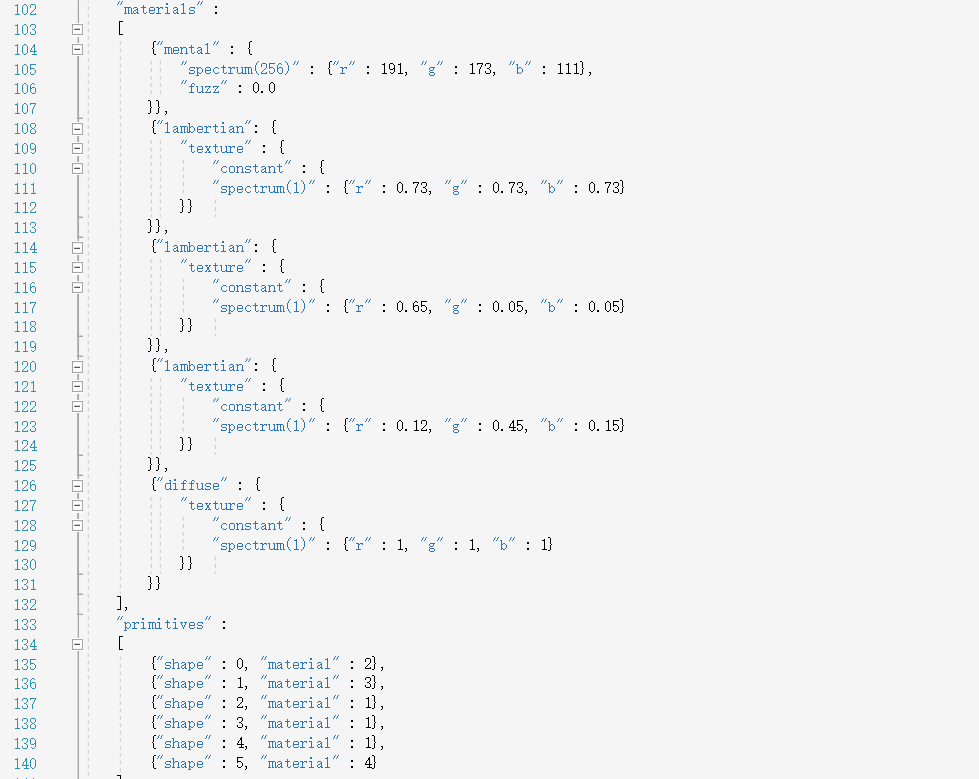
\includegraphics[scale=0.3]{code3}
\end{itemize}
\end{frame}

\begin{frame} {/core/parser.h}
\begin{itemize}
\item config对象,定义了场景输出图片的长宽和采样数
\\ camera对象,定义了场景中的相机信息
\\ transforms数组,定义了场景中所用到的转移矩阵
\\ shapes数组,定义了场景中的图形信息
\\ materials数组,定义了场景中的材质信息
\\ primitive数组,定义了场景中的图元信息
\end{itemize}
\end{frame}

\begin{frame} {/core/parser.h}
\begin{itemize}
\item \begin{semiverbatim} void load(const char *file); \end{semiverbatim}
从文件中导入JSON字符串(忽略无意义的空白符(ws))
\item \begin{semiverbatim} void run(Scene *scene); \end{semiverbatim}
开始解析入场景结构体中
\end{itemize}
\end{frame}

\begin{frame} {/core/parser.h}
\begin{itemize}
\item \begin{semiverbatim} READ\_BRACE\_BEGIN(); \end{semiverbatim}
\begin{semiverbatim} READ\_BRACE\_END(); \end{semiverbatim}
\begin{semiverbatim} READ\_COLON(); \end{semiverbatim}
\begin{semiverbatim} READ\_ARRAY\_BEGIN(); \end{semiverbatim}
\begin{semiverbatim} READ\_BRACE\_ELEMENT\_END(); \end{semiverbatim}
\begin{semiverbatim} READ\_ARRAY\_ELEMENT\_END(); \end{semiverbatim}
读入构造字符构造语法树并判断合法性, \\ 通过assert()函数检查合法性
\end{itemize}
\end{frame}

\begin{frame} {/core/parser.h}
\begin{itemize}
\item \begin{semiverbatim} std::string READ\_STRING(); \end{semiverbatim}
\begin{semiverbatim} bool READ\_BOOL(); \end{semiverbatim}
\begin{semiverbatim} int READ\_INT(); \end{semiverbatim}
\begin{semiverbatim} float READ\_FLOAT(); \end{semiverbatim}
\begin{semiverbatim} BaseVector3 READ\_VECTOR(); \end{semiverbatim}
\begin{semiverbatim} Spectrum READ\_SPECTRUM1(); \end{semiverbatim}
\begin{semiverbatim} Spectrum READ\_SPECTRUM256(); \end{semiverbatim}
读入基本的数据类型(JSON自己基础的字符串,浮点数,整数,\\ 布尔值和扩展类型,包括向量和颜色)
\end{itemize}
\end{frame}

\begin{frame} {/core/parser.h}
\begin{itemize} [<+->]
\item \begin{semiverbatim}  READ\_SHAPES(); \end{semiverbatim}
\begin{semiverbatim} READ\_SHAPE(); \end{semiverbatim}
\begin{semiverbatim} READ\_RECTANGLE(); \end{semiverbatim}
\begin{semiverbatim} READ\_SPHERE(); \end{semiverbatim}
\item 进入读取shape的分支后,先用READ\_SHAPES()对数组循环读取
\item 在循环中用READ\_SHAPE()解析其中的每个元素
\item 在解析到其中的type值对后,细化为具体 \\ READ\_RECTANGLE()或READ\_RECTANGLE()或READ\_SPHERE()的方法, \\ 进而通过读取值对读取其中的元素值
\item 其余分支读取方法相同,在此不再赘述
\end{itemize}
\end{frame}

\begin{frame} {/core/parser.h}
\begin{itemize}
\item obj文件是3D模型文件格式。适合用于3D软件模型之间的互导
\item 本项目实现了对其的读入支持
\end{itemize}
\end{frame}

\begin{frame} {Others (余畅)}
\begin{itemize} [<+->]

\item ./core/config.h 控制项目的编译选项开关
\item ./core/rng.h 实现了柏林噪声(Perlin Noise)生成器,\\ 梅森旋转(Mersenne Twister)算法实现的随机数生成器
\item ./core/memory.h 实现了自动释放和拷贝内存的引用计数指针
\item ./math/mathutility.h 使用SIMD重写了部分常用数学函数
\item ./math/bbox.h 定义了包围盒的结构体
\item ./core/primitive.h,cpp 将shape和material封装整合为图元
\item ./core/interaction.h 定义了描述相交表面细节的结构体
\item ./core/scene.h 定义了描述场景内容的结构体
\item ./core/ray.h 定义了射线的结构体
\item ./core/integrator.h 定义了对场景采样的积分器
\item ./core/spectrum.h 定义了颜色(简化后辐射度)的结构体
\end{itemize}
\end{frame}

\begin{frame} {; )}
Thank you for watching!
\end{frame}

\end{document}